% Chapter Template

\chapter{Ensayos y resultados} % Main chapter title

\label{Chapter4} % Change X to a consecutive number; for referencing this chapter elsewhere, use \ref{ChapterX}
En este capítulo se detallan los ensayos realizados para verificar el correcto funcionamiento del prototipo y el cumplimiento de los requisitos tanto en la etapa digital como en la analogica.
%----------------------------------------------------------------------------------------
%	SECTION 1
%----------------------------------------------------------------------------------------

\section{Banco de pruebas}
Para los ensayos efectuados en laboratorio se montó un banco de pruebas, figura \ref{fig:bancoDePruebas}, constituido por los siguientes elementos:

\begin{itemize}
\item Generador DDS FY6900,
\item Cable BNC-SMA (Canal descarga parcial)
\item Cable BNC-Cocodrilos (Canal senoide de referencia)
\item Computadora portátil. 
\item Puerto serie-USB
\item Prototipo funcional.
\end{itemize}

\vspace{10mm}

\begin{figure}[ht]
	\centering
	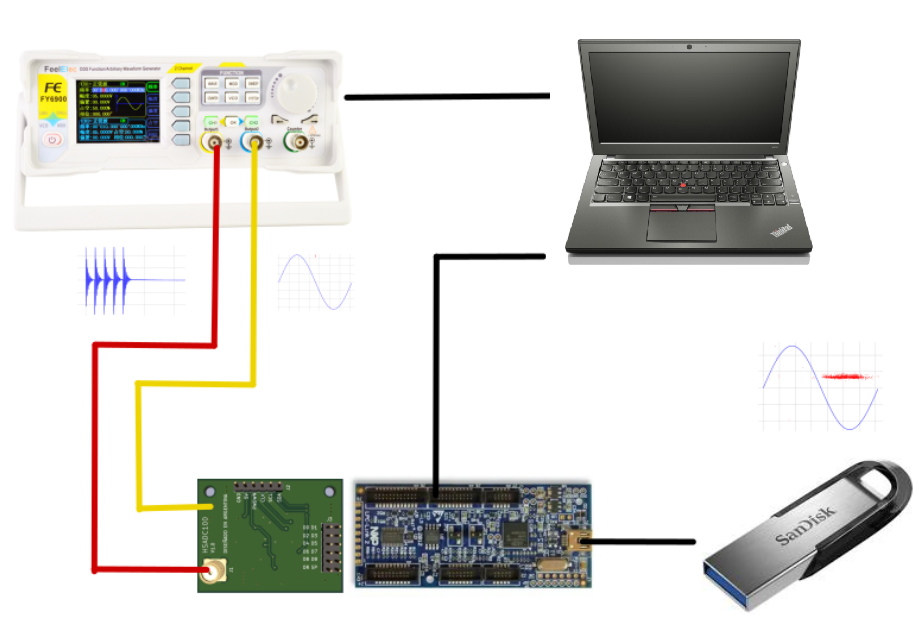
\includegraphics[width=100mm]{./Figures/bancoDePruebas.png}
	\caption{Arquitectura del banco de prueba.}
	\label{fig:bancoDePruebas}
\end{figure}

El banco permitió simular, por medio del generador, la forma de onda de una descarga parcial y sincronizarla con una senoide de referencia de 50Hz. La computadora portátil fue utilizada para acceder por medio del puerto serial a la interfaz de usuario. También se utilizó para controlar al DDS utilizando la base de datos de patrones proporcionada por el cliente. El conjunto de elementos elegidos permitió realizar diversas pruebas manuales y automatizadas.

Debido a las limitaciones del DDS FY6900 los ensayos de validación de amplitud y fase debieron hacerse por separado. Esto fue a causa de que el instrumento no permite realizar demoras en el disparo de un canal con respecto del otro.


\section{Ensayos de amplitud}
Durante los ensayos de amplitud se buscó validar que las señales obtenidas por el prototipo correspondan en amplitud y forma con la señales inyectadas. Para esto se generaron por medio del DDS señales senoidales en diferentes frecuencias y amplitudes.

En las figuras \ref{fig:sin1} y \ref{fig:sin39} se puede observar el efecto de atenuación del filtro comparando la amplitud de entrada y la amplitud medida. Las frecuencias elegidas tienen como objetivo reducir el efecto del sub muestreo cercano a la frecuencia de Nyquist que conlleva a no detectar correctamente los máximos.

\begin{figure}[ht]
	\centering
	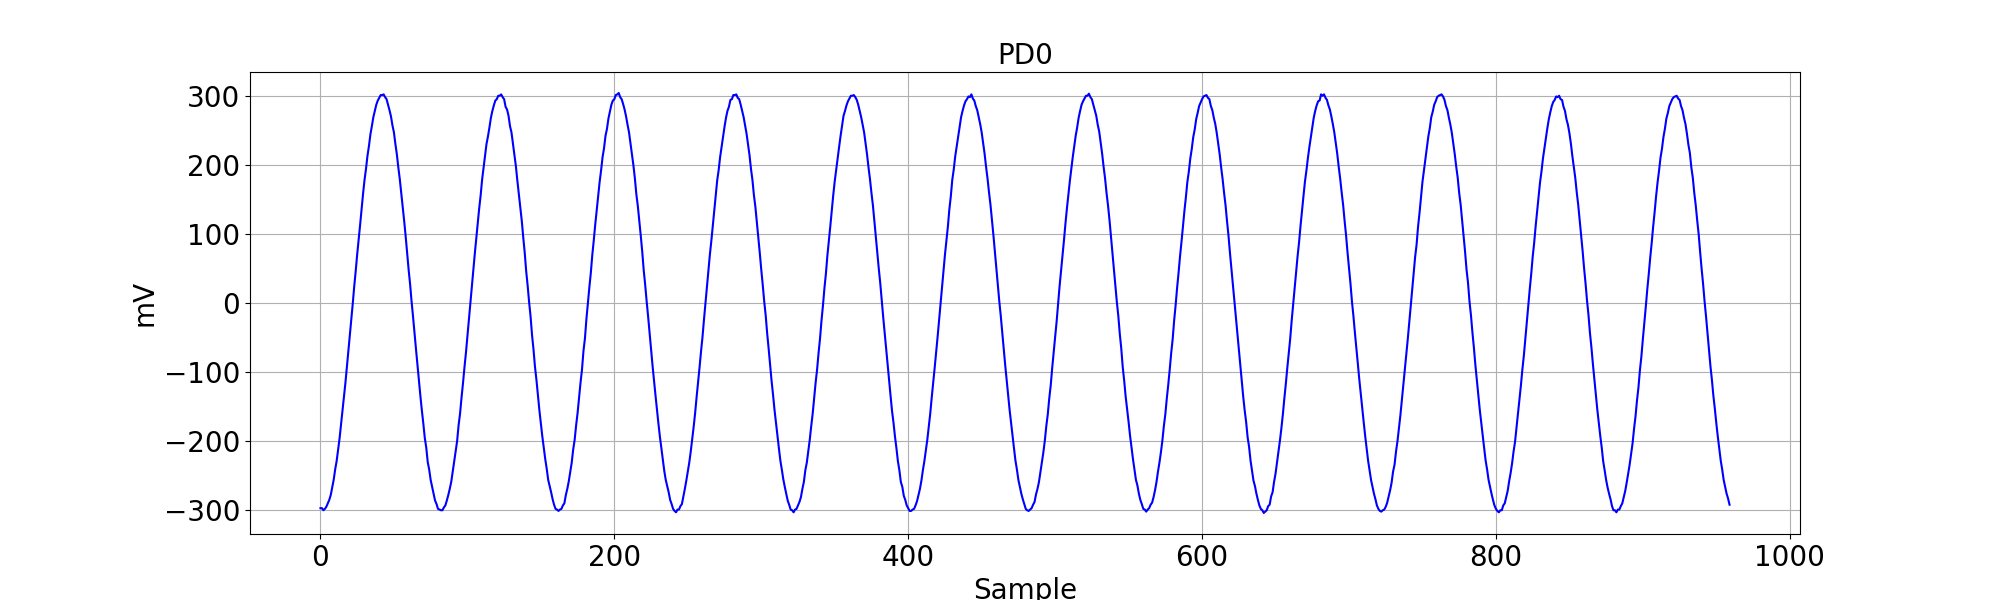
\includegraphics[width=140mm]{./Figures/sin1.png}
	\caption{Seno 1M 600 mVpp.}
	\label{fig:sin1}
\end{figure}

\begin{figure}[ht]
	\centering
	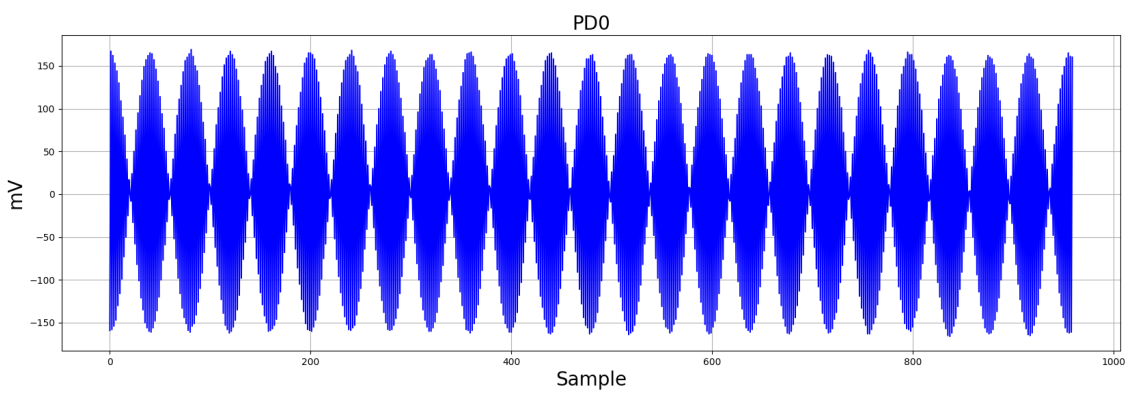
\includegraphics[width=140mm]{./Figures/sin39.png}
	\caption{Seno 39M 600 mVpp.}
	\label{fig:sin39}
\end{figure}

En la tabla se presentan la máxima tensión de entrada y la máxima tensión de salida para cada frecuencia registrada. Por medio de estos valores se calculó la respuesta en frecuencia del filtro real. 


CREAR LA TABLA

En la figura \ref{fig:respFrecReal} se puede observar la comparativa entre la respuesta del filtro esperada y la deseada

\begin{figure}[ht]
	\centering
	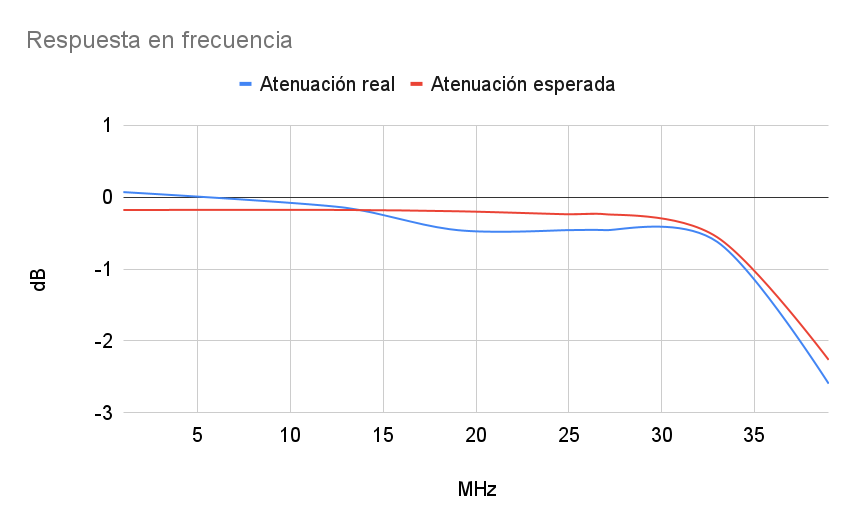
\includegraphics[width=130mm]{./Figures/respFrecReal.png}
	\caption{Respuesta en frecuencia del filtro implementado.}
	\label{fig:respFrecReal}
\end{figure}

Otra prueba realizada fue la inyección de una descarga parcial sintetizada utilizando como parámetros una descarga parcial real. En la figura \ref{fig:dpSint} puede verse la adquisición, del pulso sintetizado, realizada por el equipo.

\begin{figure}[ht]
	\centering
	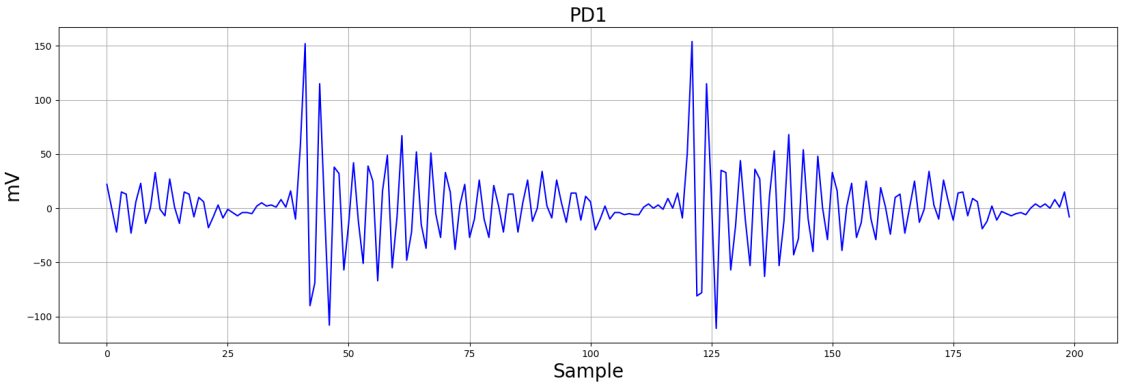
\includegraphics[width=130mm]{./Figures/dpSint.png}
	\caption{DP real sintetizada 400mvpp capturada por el equipo.}
	\label{fig:respFrecReal}
\end{figure}

La señal original fue muestreada a una tasa de 250 Msps, para poder realizar una correcta comparación de la integridad de la señal se realizó un resampling del pulso adquirido por el equipo a la misma tasa que la original. También se aplicó de forma matemática sobre la señal original la respuesta en frecuencia del filtro de entrada. Ambas señales fueron superpuestas en la figura \ref{fig:compPulsos}.

\begin{figure}[ht]
	\centering
	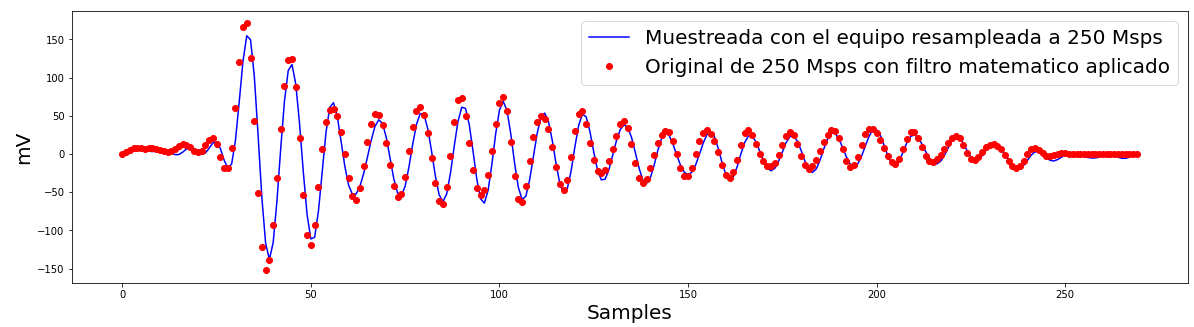
\includegraphics[width=140mm]{./Figures/compPulsos.png}
	\caption{Comparación pulso original y pulso adquirido resampleado.}
	\label{fig:compPulsos}
\end{figure}

\vspace{20mm}

Aplicando la transformada de Fourier sobre las señales de la comparativa anterior se realizó una comparativa de la distribución de energía en el espectro de la frecuencia, figura \ref{fig:compEspectro}.

\begin{figure}[ht]
	\centering
	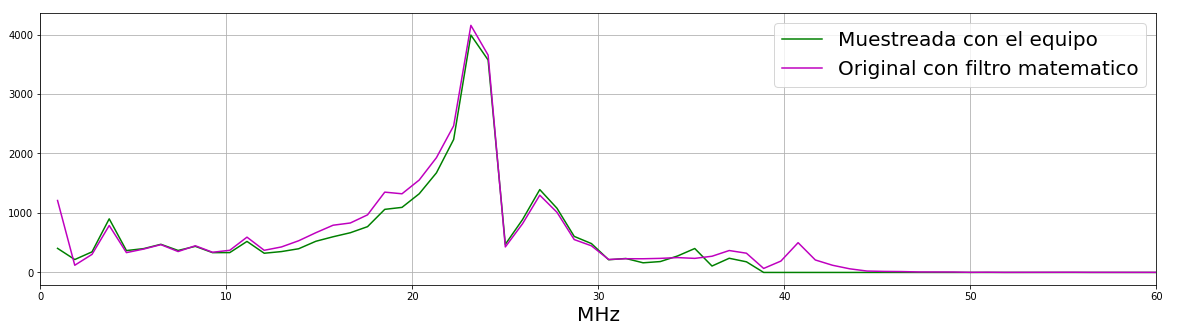
\includegraphics[width=140mm]{./Figures/compEspectro.png}
	\caption{Distribución del espectro.}
	\label{fig:compEspectro}
\end{figure}

\section{Ensayos de disparo}

\section{Ensayos de fase}

\section{Tiempos de procesamiento y almacenado}

\section{Pruebas en campo}
Debido a la pandemia global COVID-19 no fue posible realizar pruebas en campo ni en el laboratorio situado en la Universidad Tecnológica Nacional Regional General Pacheco.